\section{Event Yields and Background Estimation}
\label{sec:yields}

The results of this search in the above-mentioned kinematical region are summerized in Table~\ref{tab:ssyields1}.
As mentioned in the introduction, and quantified by this table, SM background is expected to be dominated by $t\bar{t}$ production
with one real and one fake lepton.
We estimate this background from the data itself using the ``Tight-To-Loose ratio'' (Fake Rate) method~\cite{frmethod}.
Electron charge mis-reconstruction is estimated by weighting opposite-sign dilepton events that pass all our cuts
by a charge flip rate obtained form single electron Monte Carlo as described in detail in~\cite{ssnote2011}.
The probability for muons to be reconstructed with the wrong sign in the relevant momemtum range is negligible.
Both of these techniques are described in more detail in~\cite{ssnote2011}.
Systematic errors on these two estimates are 50\% and 25\% respectively.


\newcommand{\ttdilS}{\ensuremath{\ttbar\to\ell\ell X}}
\newcommand{\ttslbS}{\ensuremath{\ttbar\to\ell(b\to\ell) X}}
\newcommand{\ttsloS}{\ensuremath{\ttbar\to\ell(b\!\!\!/\to\ell) X}}
\newcommand{\SFnn}{\ensuremath{N^{\rm Wj,raw}_{nn}}}

\begin{table}[h]
\begin{center}
\begin{tabular}{l | l l l l}
\hline\hline
 Source  &  ee  &  $\mu\mu$  &  e$\mu$  &  all \\
\hline
$t\overline{t}\rightarrow \ell\ell X$ &  0.469 $\pm$  0.305 &  0.000 $\pm$  0.199 &  1.133 $\pm$  0.580 &  1.603 $\pm$  0.656\\
$t\overline{t}$ other &  0.000 $\pm$  0.199 &  0.000 $\pm$  0.199 &  0.000 $\pm$  0.199 &  0.000 $\pm$  0.199\\
$t\overline{t}\rightarrow \ell(b\rightarrow \ell)X$ &  0.000 $\pm$  0.199 &  0.193 $\pm$  0.143 &  0.000 $\pm$  0.199 &  0.193 $\pm$  0.143\\
$t\overline{t}\rightarrow \ell(\slashed{b}\rightarrow \ell)X$ &  0.563 $\pm$  0.399 &  0.000 $\pm$  0.199 &  0.143 $\pm$  0.131 &  0.706 $\pm$  0.420\\
\hline
$t$, s-channel &  0.000 $\pm$  0.057 &  0.000 $\pm$  0.057 &  0.000 $\pm$  0.057 &  0.000 $\pm$  0.057\\
$t$, t-channel &  0.077 $\pm$  0.077 &  0.000 $\pm$  0.055 &  0.000 $\pm$  0.055 &  0.077 $\pm$  0.077\\
$tW$ &  0.000 $\pm$  0.045 &  0.000 $\pm$  0.045 &  0.016 $\pm$  0.045 &  0.016 $\pm$  0.045\\
\hline
$Z\rightarrow ee$ &  0.000 $\pm$  0.429 &  0.000 $\pm$  0.429 &  0.000 $\pm$  0.429 &  0.000 $\pm$  0.429\\
$Z\rightarrow\mu\mu$ &  0.000 $\pm$  0.429 &  0.000 $\pm$  0.429 &  0.000 $\pm$  0.429 &  0.000 $\pm$  0.429\\
$Z\rightarrow\tau\tau$ &  0.000 $\pm$  0.429 &  0.000 $\pm$  0.429 &  0.000 $\pm$  0.429 &  0.000 $\pm$  0.429\\
$W$+jets &  0.000 $\pm$  1.808 &  0.000 $\pm$  1.808 &  0.000 $\pm$  1.808 &  0.000 $\pm$  1.808\\
$WW$ &  0.000 $\pm$  0.019 &  0.000 $\pm$  0.019 &  0.000 $\pm$  0.019 &  0.000 $\pm$  0.019\\
\hline
V$\gamma$ &  0.000 $\pm$  0.248 &  0.000 $\pm$  0.248 &  0.000 $\pm$  0.248 &  0.000 $\pm$  0.248\\
$W\gamma^{*}\rightarrow\ell\nu e e$ &  0.000 $\pm$  0.097 &  0.000 $\pm$  0.097 &  0.000 $\pm$  0.097 &  0.000 $\pm$  0.097\\
$W\gamma^{*}\rightarrow\ell\nu\mu\mu$ &  0.000 $\pm$  0.075 &  0.000 $\pm$  0.075 &  0.000 $\pm$  0.075 &  0.000 $\pm$  0.075\\
$W\gamma^{*}\rightarrow\ell\nu\tau\tau$ &  0.000 $\pm$  0.028 &  0.000 $\pm$  0.028 &  0.000 $\pm$  0.028 &  0.000 $\pm$  0.028\\
$WZ$ &  0.034 $\pm$  0.012 &  0.017 $\pm$  0.008 &  0.031 $\pm$  0.012 &  0.082 $\pm$  0.019\\
$ZZ$ &   0.000 $\pm$   0.000 &  0.001 $\pm$  0.001 &  0.002 $\pm$  0.001 &  0.003 $\pm$  0.001\\
\hline
dp$W^{\pm}W^{\pm}$ &  0.000 $\pm$  0.004 &  0.000 $\pm$  0.004 &  0.000 $\pm$  0.004 &  0.000 $\pm$  0.004\\
sp$W^{-}W^{-}$ &  0.000 $\pm$  0.001 &  0.000 $\pm$  0.001 &  0.003 $\pm$  0.002 &  0.003 $\pm$  0.002\\
sp$W^{+}W^{+}$ &  0.000 $\pm$  0.006 &  0.000 $\pm$  0.006 &  0.000 $\pm$  0.006 &  0.000 $\pm$  0.006\\
$t\overline{t}\gamma$ &  0.000 $\pm$  0.059 &  0.000 $\pm$  0.059 &  0.000 $\pm$  0.059 &  0.000 $\pm$  0.059\\
$t\overline{t}W$ &  0.572 $\pm$  0.025 &  0.733 $\pm$  0.028 &  1.286 $\pm$  0.038 &  2.591 $\pm$  0.053\\
$t\overline{t}Z$ &  0.118 $\pm$  0.009 &  0.158 $\pm$  0.010 &  0.268 $\pm$  0.013 &  0.544 $\pm$  0.019\\
$WW\gamma$ &  0.000 $\pm$  0.015 &  0.000 $\pm$  0.015 &  0.000 $\pm$  0.015 &  0.000 $\pm$  0.015\\
$WWW$ &  0.001 $\pm$   0.000 &  0.001 $\pm$   0.000 &  0.001 $\pm$  0.001 &  0.003 $\pm$  0.001\\
$WWZ$ &   0.000 $\pm$   0.000 &   0.000 $\pm$   0.000 &  0.001 $\pm$  0.001 &  0.001 $\pm$  0.001\\
$WZZ$ &   0.000 $\pm$   0.000 &  0.001 $\pm$   0.000 &  0.001 $\pm$   0.000 &  0.002 $\pm$  0.001\\
$ZZZ$ &   0.000 $\pm$   0.000 &   0.000 $\pm$   0.000 &   0.000 $\pm$   0.000 &   0.000 $\pm$   0.000\\
\hline
Total MC &  1.834 $\pm$  0.509 &  1.103 $\pm$  0.146 &  2.885 $\pm$  0.597 &  5.822 $\pm$  0.797\\
\hline\hline
\hline
LM6 &  0.000 $\pm$  0.000 &  0.186 $\pm$  0.186 &  0.383 $\pm$  0.275 &  0.569 $\pm$  0.332\\
\hline\hline
\hline\hline
 SF  & 1.13 $\pm$ 0.67 & 0.30 $\pm$ 0.20 & 1.92 $\pm$ 0.74 & 3.36 $\pm$ 1.02\\
 DF  & 0.04 $\pm$ 0.12 & 0.02 $\pm$ 0.02 & 0.02 $\pm$ 0.09 & 0.08 $\pm$ 0.16\\
\hline
 SF + DF  & 1.17 $\pm$ 0.63 $\pm$ 0.58 & 0.32 $\pm$ 0.20 $\pm$ 0.16 & 1.95 $\pm$ 0.72 $\pm$ 0.97 & 3.43 $\pm$ 0.98 $\pm$ 1.72\\
\hline\hline
Charge Flips & 0.390 $\pm$ 0.032 $\pm$ 0.078 & - $\pm$ - & 0.544 $\pm$ 0.032 $\pm$ 0.109 & 0.934 $\pm$ 0.045 $\pm$ 0.187\\
\hline\hline
\hline
MC Pred &  0.725 $\pm$  0.029 $\pm$  0.362 &  0.912 $\pm$  0.031 $\pm$  0.456 &  1.595 $\pm$  0.042 $\pm$  0.797 &  3.231 $\pm$  0.059 $\pm$  1.616\\
\hline\hline
Total Pred &  2.281 $\pm$  0.633 $\pm$  0.691 &  1.232 $\pm$  0.199 $\pm$  0.483 &  4.086 $\pm$  0.725 $\pm$  1.263 &  7.600 $\pm$  0.983 $\pm$  2.365\\
\hline\hline
data & 2 & 2 & 3 & 7\\
\hline\hline
\end{tabular}

\end{center}
\caption{\label{tab:yieldBase_hpt}Observed event yields in baseline 
(\met $>$ 30 GeV, at least 2 jets with pT $>$ 40 GeV, and at least two of these jets b-tagged using SSVHEM) 
high-\pt\ (pT $>$ 20/20) dileptons
compared to expectations from simulation alone, and from the data-driven methods.
The {\em simulated backgrounds} contribution includes contributions from genuine  same-sign lepton
pairs (WZ, ZZ, leptons from same-sign W from single-parton, double-parton, and $t\bar{t}W$ production, etc.), 
as well as electrons from converted photons in $V\gamma$ production.
Entries with zero contributing events are reported with an uncertainty corresponding to one event.
This uncertainty is not added to the total MC contribution.
Systematic uncertainties (the second uncertainty if present)
 are displayed only for the final combined type of background, no systematic
uncertainty is added for estimates with zero entries.
Systematic uncertainties are 100\% correlated among the channels.
}
\end{table}

\clearpage

\begin{table}[hbt]
\begin{center}
\begin{tabular}{l | l l l l}
\hline\hline
 Source  &  ee  &  $\mu\mu$  &  e$\mu$  &  all \\
\hline
$t\overline{t}\rightarrow \ell\ell X$ &  0.069 $\pm$  0.199 &  0.000 $\pm$  0.199 &  0.000 $\pm$  0.199 &  0.069 $\pm$  0.199\\
$t\overline{t}$ other &  0.000 $\pm$  0.199 &  0.000 $\pm$  0.199 &  0.000 $\pm$  0.199 &  0.000 $\pm$  0.199\\
$t\overline{t}\rightarrow \ell(b\rightarrow \ell)X$ &  0.000 $\pm$  0.199 &  0.000 $\pm$  0.199 &  0.000 $\pm$  0.199 &  0.000 $\pm$  0.199\\
$t\overline{t}\rightarrow \ell(\slashed{b}\rightarrow \ell)X$ &  0.266 $\pm$  0.266 &  0.000 $\pm$  0.199 &  0.128 $\pm$  0.128 &  0.394 $\pm$  0.295\\
\hline
$t$, s-channel &  0.000 $\pm$  0.057 &  0.000 $\pm$  0.057 &  0.000 $\pm$  0.057 &  0.000 $\pm$  0.057\\
$t$, t-channel &  0.000 $\pm$  0.055 &  0.000 $\pm$  0.055 &  0.000 $\pm$  0.055 &  0.000 $\pm$  0.055\\
$tW$ &  0.000 $\pm$  0.045 &  0.000 $\pm$  0.045 &  0.000 $\pm$  0.045 &  0.000 $\pm$  0.045\\
\hline
$Z\rightarrow ee$ &  0.000 $\pm$  0.429 &  0.000 $\pm$  0.429 &  0.000 $\pm$  0.429 &  0.000 $\pm$  0.429\\
$Z\rightarrow\mu\mu$ &  0.000 $\pm$  0.429 &  0.000 $\pm$  0.429 &  0.000 $\pm$  0.429 &  0.000 $\pm$  0.429\\
$Z\rightarrow\tau\tau$ &  0.000 $\pm$  0.429 &  0.000 $\pm$  0.429 &  0.000 $\pm$  0.429 &  0.000 $\pm$  0.429\\
$W$+jets &  0.000 $\pm$  1.808 &  0.000 $\pm$  1.808 &  0.000 $\pm$  1.808 &  0.000 $\pm$  1.808\\
$WW$ &  0.000 $\pm$  0.019 &  0.000 $\pm$  0.019 &  0.000 $\pm$  0.019 &  0.000 $\pm$  0.019\\
\hline
V$\gamma$ &  0.000 $\pm$  0.248 &  0.000 $\pm$  0.248 &  0.000 $\pm$  0.248 &  0.000 $\pm$  0.248\\
$W\gamma^{*}\rightarrow\ell\nu e e$ &  0.000 $\pm$  0.097 &  0.000 $\pm$  0.097 &  0.000 $\pm$  0.097 &  0.000 $\pm$  0.097\\
$W\gamma^{*}\rightarrow\ell\nu\mu\mu$ &  0.000 $\pm$  0.075 &  0.000 $\pm$  0.075 &  0.000 $\pm$  0.075 &  0.000 $\pm$  0.075\\
$W\gamma^{*}\rightarrow\ell\nu\tau\tau$ &  0.000 $\pm$  0.028 &  0.000 $\pm$  0.028 &  0.000 $\pm$  0.028 &  0.000 $\pm$  0.028\\
$WZ$ &  0.009 $\pm$  0.006 &  0.001 $\pm$  0.003 &  0.006 $\pm$  0.004 &  0.016 $\pm$  0.008\\
$ZZ$ &  0.000 $\pm$   0.000 &  0.000 $\pm$   0.000 &   0.000 $\pm$   0.000 &   0.000 $\pm$   0.000\\
\hline
dp$W^{\pm}W^{\pm}$ &  0.000 $\pm$  0.004 &  0.000 $\pm$  0.004 &  0.000 $\pm$  0.004 &  0.000 $\pm$  0.004\\
sp$W^{-}W^{-}$ &  0.000 $\pm$  0.001 &  0.000 $\pm$  0.001 &  0.001 $\pm$  0.001 &  0.001 $\pm$  0.001\\
sp$W^{+}W^{+}$ &  0.000 $\pm$  0.006 &  0.000 $\pm$  0.006 &  0.000 $\pm$  0.006 &  0.000 $\pm$  0.006\\
$t\overline{t}\gamma$ &  0.000 $\pm$  0.059 &  0.000 $\pm$  0.059 &  0.000 $\pm$  0.059 &  0.000 $\pm$  0.059\\
$t\overline{t}W$ &  0.315 $\pm$  0.020 &  0.363 $\pm$  0.021 &  0.643 $\pm$  0.028 &  1.321 $\pm$  0.040\\
$t\overline{t}Z$ &  0.061 $\pm$  0.007 &  0.086 $\pm$  0.008 &  0.167 $\pm$  0.012 &  0.314 $\pm$  0.016\\
$WW\gamma$ &  0.000 $\pm$  0.015 &  0.000 $\pm$  0.015 &  0.000 $\pm$  0.015 &  0.000 $\pm$  0.015\\
$WWW$ &   0.000 $\pm$   0.000 &   0.000 $\pm$   0.000 &  0.001 $\pm$  0.001 &  0.002 $\pm$  0.001\\
$WWZ$ &  0.000 $\pm$   0.000 &  0.000 $\pm$   0.000 &  0.000 $\pm$   0.000 &  0.000 $\pm$   0.000\\
$WZZ$ &   0.000 $\pm$   0.000 &  0.000 $\pm$   0.000 &   0.000 $\pm$   0.000 &   0.000 $\pm$   0.000\\
$ZZZ$ &  0.000 $\pm$   0.000 &   0.000 $\pm$   0.000 &   0.000 $\pm$   0.000 &   0.000 $\pm$   0.000\\
\hline
Total MC &  0.721 $\pm$  0.276 &  0.451 $\pm$  0.022 &  0.946 $\pm$  0.131 &  2.118 $\pm$  0.306\\
\hline\hline
\hline
LM6 &  0.000 $\pm$  0.000 &  0.000 $\pm$  0.000 &  0.000 $\pm$  0.000 &  0.000 $\pm$  0.000\\
\hline\hline
\hline\hline
 SF  & 0.27 $\pm$ 0.54 & 0.00 $\pm$ 0.37 & 0.54 $\pm$ 0.59 & 0.81 $\pm$ 0.74\\
 DF  & 0.00 $\pm$ 0.14 & 0.00 $\pm$ 0.10 & 0.00 $\pm$ 0.16 & 0.00 $\pm$ 0.16\\
\hline
 SF + DF  & 0.27 $\pm$ 0.45 $\pm$ 0.14 & 0.00 $\pm$ 0.31 $\pm$ 0.00 & 0.54 $\pm$ 0.50 $\pm$ 0.27 & 0.81 $\pm$ 0.67 $\pm$ 0.40\\
\hline\hline
Charge Flips & 0.036 $\pm$ 0.010 $\pm$ 0.007 & - $\pm$ - & 0.069 $\pm$ 0.012 $\pm$ 0.014 & 0.104 $\pm$ 0.015 $\pm$ 0.021\\
\hline\hline
\hline
MC Pred &  0.386 $\pm$  0.022 $\pm$  0.193 &  0.451 $\pm$  0.022 $\pm$  0.225 &  0.818 $\pm$  0.031 $\pm$  0.409 &  1.655 $\pm$  0.044 $\pm$  0.827\\
\hline\hline
Total Pred &  0.695 $\pm$  0.453 $\pm$  0.236 &  0.451 $\pm$  0.315 $\pm$  0.225 &  1.422 $\pm$  0.496 $\pm$  0.489 &  2.568 $\pm$  0.672 $\pm$  0.921\\
\hline\hline
data & 1 & 1 & 0 & 2\\
\hline\hline
\end{tabular}

\end{center}
\caption{\label{tab:yieldlom0_hpt}Observed event yields in high-\pt\ (pT $>$ 20/20) dileptons
passing the {\em low-$m_0$} signal selections ($H_T > $ 320 GeV, \met $>$ 50 GeV)
compared to expectations from simulation alone, and from the data-driven methods.
The {\em simulated backgrounds} contribution includes contributions from genuine  same-sign lepton
pairs (WZ, ZZ, leptons from same-sign W from single-, double-parton, and $t\bar{t}W$ production, etc.), 
as well as electrons from converted photons in $V\gamma$ production.
Entries with zero contributing events are reported with an uncertainty corresponding to one event.
This uncertainty is not added to the total MC contribution.
Systematic uncertainties (the second uncertainty if present)
 are displayed only for the final combined type of background, no systematic
uncertainty is added for estimates with zero entries.
Systematic uncertainties are 100\% correlated among the channels.
}
\end{table}
\clearpage

\begin{table}[hbt]
\begin{center}
\begin{tabular}{l | l l l l}
\hline\hline
 Source  &  ee  &  $\mu\mu$  &  e$\mu$  &  all \\
\hline
$t\overline{t}\rightarrow \ell\ell X$ &  0.000 $\pm$  0.199 &  0.000 $\pm$  0.199 &  0.000 $\pm$  0.199 &  0.000 $\pm$  0.199\\
$t\overline{t}$ other &  0.000 $\pm$  0.199 &  0.000 $\pm$  0.199 &  0.000 $\pm$  0.199 &  0.000 $\pm$  0.199\\
$t\overline{t}\rightarrow \ell(b\rightarrow \ell)X$ &  0.000 $\pm$  0.199 &  0.000 $\pm$  0.199 &  0.000 $\pm$  0.199 &  0.000 $\pm$  0.199\\
$t\overline{t}\rightarrow \ell(\slashed{b}\rightarrow \ell)X$ &  0.266 $\pm$  0.266 &  0.000 $\pm$  0.199 &  0.000 $\pm$  0.199 &  0.266 $\pm$  0.266\\
\hline
$t$, s-channel &  0.000 $\pm$  0.057 &  0.000 $\pm$  0.057 &  0.000 $\pm$  0.057 &  0.000 $\pm$  0.057\\
$t$, t-channel &  0.000 $\pm$  0.055 &  0.000 $\pm$  0.055 &  0.000 $\pm$  0.055 &  0.000 $\pm$  0.055\\
$tW$ &  0.000 $\pm$  0.045 &  0.000 $\pm$  0.045 &  0.000 $\pm$  0.045 &  0.000 $\pm$  0.045\\
\hline
$Z\rightarrow ee$ &  0.000 $\pm$  0.429 &  0.000 $\pm$  0.429 &  0.000 $\pm$  0.429 &  0.000 $\pm$  0.429\\
$Z\rightarrow\mu\mu$ &  0.000 $\pm$  0.429 &  0.000 $\pm$  0.429 &  0.000 $\pm$  0.429 &  0.000 $\pm$  0.429\\
$Z\rightarrow\tau\tau$ &  0.000 $\pm$  0.429 &  0.000 $\pm$  0.429 &  0.000 $\pm$  0.429 &  0.000 $\pm$  0.429\\
$W$+jets &  0.000 $\pm$  1.808 &  0.000 $\pm$  1.808 &  0.000 $\pm$  1.808 &  0.000 $\pm$  1.808\\
$WW$ &  0.000 $\pm$  0.019 &  0.000 $\pm$  0.019 &  0.000 $\pm$  0.019 &  0.000 $\pm$  0.019\\
\hline
V$\gamma$ &  0.000 $\pm$  0.248 &  0.000 $\pm$  0.248 &  0.000 $\pm$  0.248 &  0.000 $\pm$  0.248\\
$W\gamma^{*}\rightarrow\ell\nu e e$ &  0.000 $\pm$  0.097 &  0.000 $\pm$  0.097 &  0.000 $\pm$  0.097 &  0.000 $\pm$  0.097\\
$W\gamma^{*}\rightarrow\ell\nu\mu\mu$ &  0.000 $\pm$  0.075 &  0.000 $\pm$  0.075 &  0.000 $\pm$  0.075 &  0.000 $\pm$  0.075\\
$W\gamma^{*}\rightarrow\ell\nu\tau\tau$ &  0.000 $\pm$  0.028 &  0.000 $\pm$  0.028 &  0.000 $\pm$  0.028 &  0.000 $\pm$  0.028\\
$WZ$ &  0.000 $\pm$  0.003 &  0.001 $\pm$  0.003 &  0.004 $\pm$  0.004 &  0.005 $\pm$  0.004\\
$ZZ$ &  0.000 $\pm$   0.000 &  0.000 $\pm$   0.000 &  0.000 $\pm$   0.000 &  0.000 $\pm$   0.000\\
\hline
dp$W^{\pm}W^{\pm}$ &  0.000 $\pm$  0.004 &  0.000 $\pm$  0.004 &  0.000 $\pm$  0.004 &  0.000 $\pm$  0.004\\
sp$W^{-}W^{-}$ &  0.000 $\pm$  0.001 &  0.000 $\pm$  0.001 &  0.001 $\pm$  0.001 &  0.001 $\pm$  0.001\\
sp$W^{+}W^{+}$ &  0.000 $\pm$  0.006 &  0.000 $\pm$  0.006 &  0.000 $\pm$  0.006 &  0.000 $\pm$  0.006\\
$t\overline{t}\gamma$ &  0.000 $\pm$  0.059 &  0.000 $\pm$  0.059 &  0.000 $\pm$  0.059 &  0.000 $\pm$  0.059\\
$t\overline{t}W$ &  0.143 $\pm$  0.013 &  0.168 $\pm$  0.014 &  0.302 $\pm$  0.019 &  0.614 $\pm$  0.027\\
$t\overline{t}Z$ &  0.031 $\pm$  0.005 &  0.046 $\pm$  0.006 &  0.091 $\pm$  0.008 &  0.168 $\pm$  0.011\\
$WW\gamma$ &  0.000 $\pm$  0.015 &  0.000 $\pm$  0.015 &  0.000 $\pm$  0.015 &  0.000 $\pm$  0.015\\
$WWW$ &   0.000 $\pm$   0.000 &   0.000 $\pm$   0.000 &  0.001 $\pm$   0.000 &  0.001 $\pm$  0.001\\
$WWZ$ &  0.000 $\pm$   0.000 &  0.000 $\pm$   0.000 &  0.000 $\pm$   0.000 &  0.000 $\pm$   0.000\\
$WZZ$ &  0.000 $\pm$   0.000 &  0.000 $\pm$   0.000 &  0.000 $\pm$   0.000 &  0.000 $\pm$   0.000\\
$ZZZ$ &  0.000 $\pm$   0.000 &  0.000 $\pm$   0.000 &  0.000 $\pm$   0.000 &  0.000 $\pm$   0.000\\
\hline
Total MC &  0.441 $\pm$  0.267 &  0.216 $\pm$  0.015 &  0.400 $\pm$  0.021 &  1.056 $\pm$  0.268\\
\hline\hline
\hline
LM6 &  0.000 $\pm$  0.000 &  0.000 $\pm$  0.000 &  0.000 $\pm$  0.000 &  0.000 $\pm$  0.000\\
\hline\hline
\hline\hline
 SF  & 0.00 $\pm$ 0.58 & 0.00 $\pm$ 0.37 & 0.15 $\pm$ 0.54 & 0.15 $\pm$ 0.54\\
 DF  & 0.00 $\pm$ 0.14 & 0.00 $\pm$ 0.10 & 0.00 $\pm$ 0.16 & 0.00 $\pm$ 0.16\\
\hline
 SF + DF  & 0.00 $\pm$ 0.50 $\pm$ 0.00 & 0.00 $\pm$ 0.31 $\pm$ 0.00 & 0.15 $\pm$ 0.44 $\pm$ 0.07 & 0.15 $\pm$ 0.44 $\pm$ 0.07\\
\hline\hline
Charge Flips & 0.011 $\pm$ 0.004 $\pm$ 0.002 & - $\pm$ - & 0.016 $\pm$ 0.005 $\pm$ 0.003 & 0.027 $\pm$ 0.006 $\pm$ 0.005\\
\hline\hline
\hline
MC Pred &  0.175 $\pm$  0.014 $\pm$  0.087 &  0.216 $\pm$  0.015 $\pm$  0.108 &  0.400 $\pm$  0.021 $\pm$  0.200 &  0.790 $\pm$  0.030 $\pm$  0.395\\
\hline\hline
Total Pred &  0.186 $\pm$  0.501 $\pm$  0.087 &  0.216 $\pm$  0.315 $\pm$  0.108 &  0.565 $\pm$  0.438 $\pm$  0.213 &  0.966 $\pm$  0.439 $\pm$  0.402\\
\hline\hline
data & 1 & 0 & 0 & 1\\
\hline\hline
\end{tabular}

\end{center}
\caption{\label{tab:yieldhim0_hpt}Observed event yields in high-\pt\ (pT $>$ 20/20) dileptons
passing the {\em high-$m_0$} signal selections ($H_T > 440$ GeV, \met $>$ 50 GeV)
compared to expectations from simulation alone, and from the data-driven methods.
The {\em simulated backgrounds} contribution includes contributions from genuine  same-sign lepton
pairs (WZ, ZZ, leptons from same-sign W from single-, double-parton, and $t\bar{t}W$ production, etc.), 
as well as electrons from converted photons in $V\gamma$ production.
Entries with zero contributing events are reported with an uncertainty corresponding to one event.
This uncertainty is not added to the total MC contribution.
Systematic uncertainties (the second uncertainty if present)
 are displayed only for the final combined type of background, no systematic
uncertainty is added for estimates with zero entries.
Systematic uncertainties are 100\% correlated among the channels.
}
\end{table}
\clearpage

\begin{table}[hbt]
\begin{center}
\begin{tabular}{l | l l l l}
\hline\hline
 Source  &  ee  &  $\mu\mu$  &  e$\mu$  &  all \\
\hline
$t\overline{t}\rightarrow \ell\ell X$ &  0.000 $\pm$  0.199 &  0.000 $\pm$  0.199 &  0.000 $\pm$  0.199 &  0.000 $\pm$  0.199\\
$t\overline{t}$ other &  0.000 $\pm$  0.199 &  0.000 $\pm$  0.199 &  0.000 $\pm$  0.199 &  0.000 $\pm$  0.199\\
$t\overline{t}\rightarrow \ell(b\rightarrow \ell)X$ &  0.000 $\pm$  0.199 &  0.000 $\pm$  0.199 &  0.000 $\pm$  0.199 &  0.000 $\pm$  0.199\\
$t\overline{t}\rightarrow \ell(\slashed{b}\rightarrow \ell)X$ &  0.000 $\pm$  0.199 &  0.000 $\pm$  0.199 &  0.000 $\pm$  0.199 &  0.000 $\pm$  0.199\\
\hline
$t$, s-channel &  0.000 $\pm$  0.057 &  0.000 $\pm$  0.057 &  0.000 $\pm$  0.057 &  0.000 $\pm$  0.057\\
$t$, t-channel &  0.000 $\pm$  0.055 &  0.000 $\pm$  0.055 &  0.000 $\pm$  0.055 &  0.000 $\pm$  0.055\\
$tW$ &  0.000 $\pm$  0.045 &  0.000 $\pm$  0.045 &  0.000 $\pm$  0.045 &  0.000 $\pm$  0.045\\
\hline
$Z\rightarrow ee$ &  0.000 $\pm$  0.429 &  0.000 $\pm$  0.429 &  0.000 $\pm$  0.429 &  0.000 $\pm$  0.429\\
$Z\rightarrow\mu\mu$ &  0.000 $\pm$  0.429 &  0.000 $\pm$  0.429 &  0.000 $\pm$  0.429 &  0.000 $\pm$  0.429\\
$Z\rightarrow\tau\tau$ &  0.000 $\pm$  0.429 &  0.000 $\pm$  0.429 &  0.000 $\pm$  0.429 &  0.000 $\pm$  0.429\\
$W$+jets &  0.000 $\pm$  1.808 &  0.000 $\pm$  1.808 &  0.000 $\pm$  1.808 &  0.000 $\pm$  1.808\\
$WW$ &  0.000 $\pm$  0.019 &  0.000 $\pm$  0.019 &  0.000 $\pm$  0.019 &  0.000 $\pm$  0.019\\
\hline
V$\gamma$ &  0.000 $\pm$  0.248 &  0.000 $\pm$  0.248 &  0.000 $\pm$  0.248 &  0.000 $\pm$  0.248\\
$W\gamma^{*}\rightarrow\ell\nu e e$ &  0.000 $\pm$  0.097 &  0.000 $\pm$  0.097 &  0.000 $\pm$  0.097 &  0.000 $\pm$  0.097\\
$W\gamma^{*}\rightarrow\ell\nu\mu\mu$ &  0.000 $\pm$  0.075 &  0.000 $\pm$  0.075 &  0.000 $\pm$  0.075 &  0.000 $\pm$  0.075\\
$W\gamma^{*}\rightarrow\ell\nu\tau\tau$ &  0.000 $\pm$  0.028 &  0.000 $\pm$  0.028 &  0.000 $\pm$  0.028 &  0.000 $\pm$  0.028\\
$WZ$ &  0.005 $\pm$  0.005 &  0.000 $\pm$  0.003 &  0.000 $\pm$  0.003 &  0.005 $\pm$  0.005\\
$ZZ$ &  0.000 $\pm$   0.000 &  0.000 $\pm$   0.000 &   0.000 $\pm$   0.000 &   0.000 $\pm$   0.000\\
\hline
dp$W^{\pm}W^{\pm}$ &  0.000 $\pm$  0.004 &  0.000 $\pm$  0.004 &  0.000 $\pm$  0.004 &  0.000 $\pm$  0.004\\
sp$W^{-}W^{-}$ &  0.000 $\pm$  0.001 &  0.000 $\pm$  0.001 &  0.000 $\pm$  0.001 &  0.000 $\pm$  0.001\\
sp$W^{+}W^{+}$ &  0.000 $\pm$  0.006 &  0.000 $\pm$  0.006 &  0.000 $\pm$  0.006 &  0.000 $\pm$  0.006\\
$t\overline{t}\gamma$ &  0.000 $\pm$  0.059 &  0.000 $\pm$  0.059 &  0.000 $\pm$  0.059 &  0.000 $\pm$  0.059\\
$t\overline{t}W$ &  0.028 $\pm$  0.006 &  0.041 $\pm$  0.006 &  0.076 $\pm$  0.009 &  0.145 $\pm$  0.012\\
$t\overline{t}Z$ &  0.003 $\pm$  0.001 &  0.009 $\pm$  0.003 &  0.008 $\pm$  0.002 &  0.020 $\pm$  0.004\\
$WW\gamma$ &  0.000 $\pm$  0.015 &  0.000 $\pm$  0.015 &  0.000 $\pm$  0.015 &  0.000 $\pm$  0.015\\
$WWW$ &   0.000 $\pm$   0.000 &  0.000 $\pm$   0.000 &   0.000 $\pm$   0.000 &   0.000 $\pm$   0.000\\
$WWZ$ &  0.000 $\pm$   0.000 &  0.000 $\pm$   0.000 &  0.000 $\pm$   0.000 &  0.000 $\pm$   0.000\\
$WZZ$ &  0.000 $\pm$   0.000 &  0.000 $\pm$   0.000 &  0.000 $\pm$   0.000 &  0.000 $\pm$   0.000\\
$ZZZ$ &  0.000 $\pm$   0.000 &  0.000 $\pm$   0.000 &   0.000 $\pm$   0.000 &   0.000 $\pm$   0.000\\
\hline
Total MC &  0.036 $\pm$  0.008 &  0.049 $\pm$  0.007 &  0.085 $\pm$  0.009 &  0.170 $\pm$  0.014\\
\hline\hline
\hline
LM6 &  0.000 $\pm$  0.000 &  0.000 $\pm$  0.000 &  0.000 $\pm$  0.000 &  0.000 $\pm$  0.000\\
\hline\hline
\hline\hline
 SF  & 0.00 $\pm$ 0.58 & 0.00 $\pm$ 0.37 & 0.18 $\pm$ 0.55 & 0.18 $\pm$ 0.55\\
 DF  & 0.00 $\pm$ 0.14 & 0.00 $\pm$ 0.10 & 0.00 $\pm$ 0.16 & 0.00 $\pm$ 0.16\\
\hline
 SF + DF  & 0.00 $\pm$ 0.50 $\pm$ 0.00 & 0.00 $\pm$ 0.31 $\pm$ 0.00 & 0.18 $\pm$ 0.45 $\pm$ 0.09 & 0.18 $\pm$ 0.45 $\pm$ 0.09\\
\hline\hline
Charge Flips & 0.007 $\pm$ 0.003 $\pm$ 0.001 & - $\pm$ - & 0.010 $\pm$ 0.004 $\pm$ 0.002 & 0.017 $\pm$ 0.005 $\pm$ 0.003\\
\hline\hline
\hline
MC Pred &  0.036 $\pm$  0.008 $\pm$  0.018 &  0.049 $\pm$  0.007 $\pm$  0.025 &  0.085 $\pm$  0.009 $\pm$  0.042 &  0.170 $\pm$  0.014 $\pm$  0.085\\
\hline\hline
Total Pred &  0.043 $\pm$  0.501 $\pm$  0.018 &  0.049 $\pm$  0.315 $\pm$  0.025 &  0.270 $\pm$  0.447 $\pm$  0.097 &  0.363 $\pm$  0.447 $\pm$  0.122\\
\hline\hline
data & 1 & 0 & 1 & 2\\
\hline\hline
\end{tabular}

\end{center}
\caption{\label{tab:yieldsimple_hpt}Observed event yields in high-\pt\ (pT $>$ 20/20) dileptons
passing the {\em simplified model} signal selections ($H_T > 200$ GeV, \met $>$ 120 GeV)
compared to expectations from simulation alone, and from the data-driven methods.
The {\em simulated backgrounds} contribution includes contributions from genuine  same-sign lepton
pairs (WZ, ZZ, leptons from same-sign W from single-, double-parton, and $t\bar{t}W$ production, etc.), 
as well as electrons from converted photons in $V\gamma$ production.
Entries with zero contributing events are reported with an uncertainty corresponding to one event.
This uncertainty is not added to the total MC contribution.
Systematic uncertainties (the second uncertainty if present)
 are displayed only for the final combined type of background, no systematic
uncertainty is added for estimates with zero entries.
Systematic uncertainties are 100\% correlated among the channels.
}
\end{table}

\clearpage

\begin{table}[hbt]
\begin{center}
\begin{tabular}{l | l l l l}
\hline\hline
 Source  &  ee  &  $\mu\mu$  &  e$\mu$  &  all \\
\hline
$t\overline{t}\rightarrow \ell\ell X$ &  0.000 $\pm$  0.199 &  0.000 $\pm$  0.199 &  0.000 $\pm$  0.199 &  0.000 $\pm$  0.199\\
$t\overline{t}$ other &  0.000 $\pm$  0.199 &  0.000 $\pm$  0.199 &  0.000 $\pm$  0.199 &  0.000 $\pm$  0.199\\
$t\overline{t}\rightarrow \ell(b\rightarrow \ell)X$ &  0.000 $\pm$  0.199 &  0.000 $\pm$  0.199 &  0.000 $\pm$  0.199 &  0.000 $\pm$  0.199\\
$t\overline{t}\rightarrow \ell(\slashed{b}\rightarrow \ell)X$ &  0.000 $\pm$  0.199 &  0.000 $\pm$  0.199 &  0.000 $\pm$  0.199 &  0.000 $\pm$  0.199\\
\hline
$t$, s-channel &  0.000 $\pm$  0.057 &  0.000 $\pm$  0.057 &  0.000 $\pm$  0.057 &  0.000 $\pm$  0.057\\
$t$, t-channel &  0.000 $\pm$  0.055 &  0.000 $\pm$  0.055 &  0.000 $\pm$  0.055 &  0.000 $\pm$  0.055\\
$tW$ &  0.000 $\pm$  0.045 &  0.000 $\pm$  0.045 &  0.000 $\pm$  0.045 &  0.000 $\pm$  0.045\\
\hline
$Z\rightarrow ee$ &  0.000 $\pm$  0.429 &  0.000 $\pm$  0.429 &  0.000 $\pm$  0.429 &  0.000 $\pm$  0.429\\
$Z\rightarrow\mu\mu$ &  0.000 $\pm$  0.429 &  0.000 $\pm$  0.429 &  0.000 $\pm$  0.429 &  0.000 $\pm$  0.429\\
$Z\rightarrow\tau\tau$ &  0.000 $\pm$  0.429 &  0.000 $\pm$  0.429 &  0.000 $\pm$  0.429 &  0.000 $\pm$  0.429\\
$W$+jets &  0.000 $\pm$  1.808 &  0.000 $\pm$  1.808 &  0.000 $\pm$  1.808 &  0.000 $\pm$  1.808\\
$WW$ &  0.000 $\pm$  0.019 &  0.000 $\pm$  0.019 &  0.000 $\pm$  0.019 &  0.000 $\pm$  0.019\\
\hline
V$\gamma$ &  0.000 $\pm$  0.248 &  0.000 $\pm$  0.248 &  0.000 $\pm$  0.248 &  0.000 $\pm$  0.248\\
$W\gamma^{*}\rightarrow\ell\nu e e$ &  0.000 $\pm$  0.097 &  0.000 $\pm$  0.097 &  0.000 $\pm$  0.097 &  0.000 $\pm$  0.097\\
$W\gamma^{*}\rightarrow\ell\nu\mu\mu$ &  0.000 $\pm$  0.075 &  0.000 $\pm$  0.075 &  0.000 $\pm$  0.075 &  0.000 $\pm$  0.075\\
$W\gamma^{*}\rightarrow\ell\nu\tau\tau$ &  0.000 $\pm$  0.028 &  0.000 $\pm$  0.028 &  0.000 $\pm$  0.028 &  0.000 $\pm$  0.028\\
$WZ$ &  0.004 $\pm$  0.004 &  0.001 $\pm$  0.003 &   0.000 $\pm$  0.003 &  0.006 $\pm$  0.005\\
$ZZ$ &  0.000 $\pm$   0.000 &  0.000 $\pm$   0.000 &   0.000 $\pm$   0.000 &   0.000 $\pm$   0.000\\
\hline
dp$W^{\pm}W^{\pm}$ &  0.000 $\pm$  0.004 &  0.000 $\pm$  0.004 &  0.000 $\pm$  0.004 &  0.000 $\pm$  0.004\\
sp$W^{-}W^{-}$ &  0.000 $\pm$  0.001 &  0.000 $\pm$  0.001 &  0.001 $\pm$  0.001 &  0.001 $\pm$  0.001\\
sp$W^{+}W^{+}$ &  0.000 $\pm$  0.006 &  0.000 $\pm$  0.006 &  0.000 $\pm$  0.006 &  0.000 $\pm$  0.006\\
$t\overline{t}\gamma$ &  0.000 $\pm$  0.059 &  0.000 $\pm$  0.059 &  0.000 $\pm$  0.059 &  0.000 $\pm$  0.059\\
$t\overline{t}W$ &  0.117 $\pm$  0.012 &  0.141 $\pm$  0.013 &  0.250 $\pm$  0.017 &  0.508 $\pm$  0.025\\
$t\overline{t}Z$ &  0.017 $\pm$  0.004 &  0.026 $\pm$  0.004 &  0.053 $\pm$  0.007 &  0.096 $\pm$  0.009\\
$WW\gamma$ &  0.000 $\pm$  0.015 &  0.000 $\pm$  0.015 &  0.000 $\pm$  0.015 &  0.000 $\pm$  0.015\\
$WWW$ &  0.000 $\pm$   0.000 &   0.000 $\pm$   0.000 &   0.000 $\pm$   0.000 &   0.000 $\pm$   0.000\\
$WWZ$ &  0.000 $\pm$   0.000 &  0.000 $\pm$   0.000 &  0.000 $\pm$   0.000 &  0.000 $\pm$   0.000\\
$WZZ$ &   0.000 $\pm$   0.000 &  0.000 $\pm$   0.000 &   0.000 $\pm$   0.000 &   0.000 $\pm$   0.000\\
$ZZZ$ &  0.000 $\pm$   0.000 &  0.000 $\pm$   0.000 &  0.000 $\pm$   0.000 &  0.000 $\pm$   0.000\\
\hline
Total MC &  0.138 $\pm$  0.013 &  0.168 $\pm$  0.014 &  0.305 $\pm$  0.019 &  0.611 $\pm$  0.027\\
\hline\hline
\hline
LM6 &  0.000 $\pm$  0.000 &  0.000 $\pm$  0.000 &  0.000 $\pm$  0.000 &  0.000 $\pm$  0.000\\
\hline\hline
\hline\hline
 SF  & 0.00 $\pm$ 0.58 & 0.00 $\pm$ 0.37 & 0.15 $\pm$ 0.54 & 0.15 $\pm$ 0.54\\
 DF  & 0.00 $\pm$ 0.14 & 0.00 $\pm$ 0.10 & 0.00 $\pm$ 0.16 & 0.00 $\pm$ 0.16\\
\hline
 SF + DF  & 0.00 $\pm$ 0.50 $\pm$ 0.00 & 0.00 $\pm$ 0.31 $\pm$ 0.00 & 0.15 $\pm$ 0.44 $\pm$ 0.07 & 0.15 $\pm$ 0.44 $\pm$ 0.07\\
\hline\hline
Charge Flips & 0.014 $\pm$ 0.006 $\pm$ 0.003 & - $\pm$ - & 0.011 $\pm$ 0.005 $\pm$ 0.002 & 0.025 $\pm$ 0.008 $\pm$ 0.005\\
\hline\hline
\hline
MC Pred &  0.138 $\pm$  0.013 $\pm$  0.069 &  0.168 $\pm$  0.014 $\pm$  0.084 &  0.305 $\pm$  0.019 $\pm$  0.153 &  0.612 $\pm$  0.027 $\pm$  0.306\\
\hline\hline
Total Pred &  0.152 $\pm$  0.501 $\pm$  0.069 &  0.168 $\pm$  0.315 $\pm$  0.084 &  0.466 $\pm$  0.438 $\pm$  0.170 &  0.787 $\pm$  0.439 $\pm$  0.315\\
\hline\hline
data & 0 & 0 & 0 & 0\\
\hline\hline
\end{tabular}

\end{center}
\caption{\label{tab:yieldsnu_hpt}Observed event yields in high-\pt\ (pT $>$ 20/20) dileptons
passing the {\em pMSSW/sneutrino} signal selections ($H_T > 320$ GeV, \met $>$ 120 GeV)
compared to expectations from simulation alone, and from the data-driven methods.
The {\em simulated backgrounds} contribution includes contributions from genuine  same-sign lepton
pairs (WZ, ZZ, leptons from same-sign W from single-, double-parton, and $t\bar{t}W$ production, etc.), 
as well as electrons from converted photons in $V\gamma$ production.
Entries with zero contributing events are reported with an uncertainty corresponding to one event.
This uncertainty is not added to the total MC contribution.
Systematic uncertainties (the second uncertainty if present)
 are displayed only for the final combined type of background, no systematic
uncertainty is added for estimates with zero entries.
Systematic uncertainties are 100\% correlated among the channels.
}
\end{table}

\clearpage

The estimation
is in a good agreement with the observation. 
We also note that the backgrounds with respect to the inclusive same-sign
dilepton search is suppressed by an order of magnitude due to the b-tag requirements.
As seen in the yield tables above, the contribution from fake leptons from $b$-quark decays in \ttbar,
which is the dominant in the pre-tagged sample analysis~\cite{ssnote2011},
is now suppressed and is no longer a dominant one.
This confirms our initial expectation from requiring two b-tagged jets.




%%Finally, Figure~\ref{fig:ttbar_residual} shows the minimum $\Delta R$ between one of the two b-tagged jets and 
%%the fake lepton in the MC after 
%%relaxing the jet veto cone around the lepton. 
%%The black line indicates the jet veto cone size. Clearly, a b-quark can not simultaneously provide a b-tag and an isolated lepton.
%%
%%\begin{figure}[htb]
%%\begin{center}
%%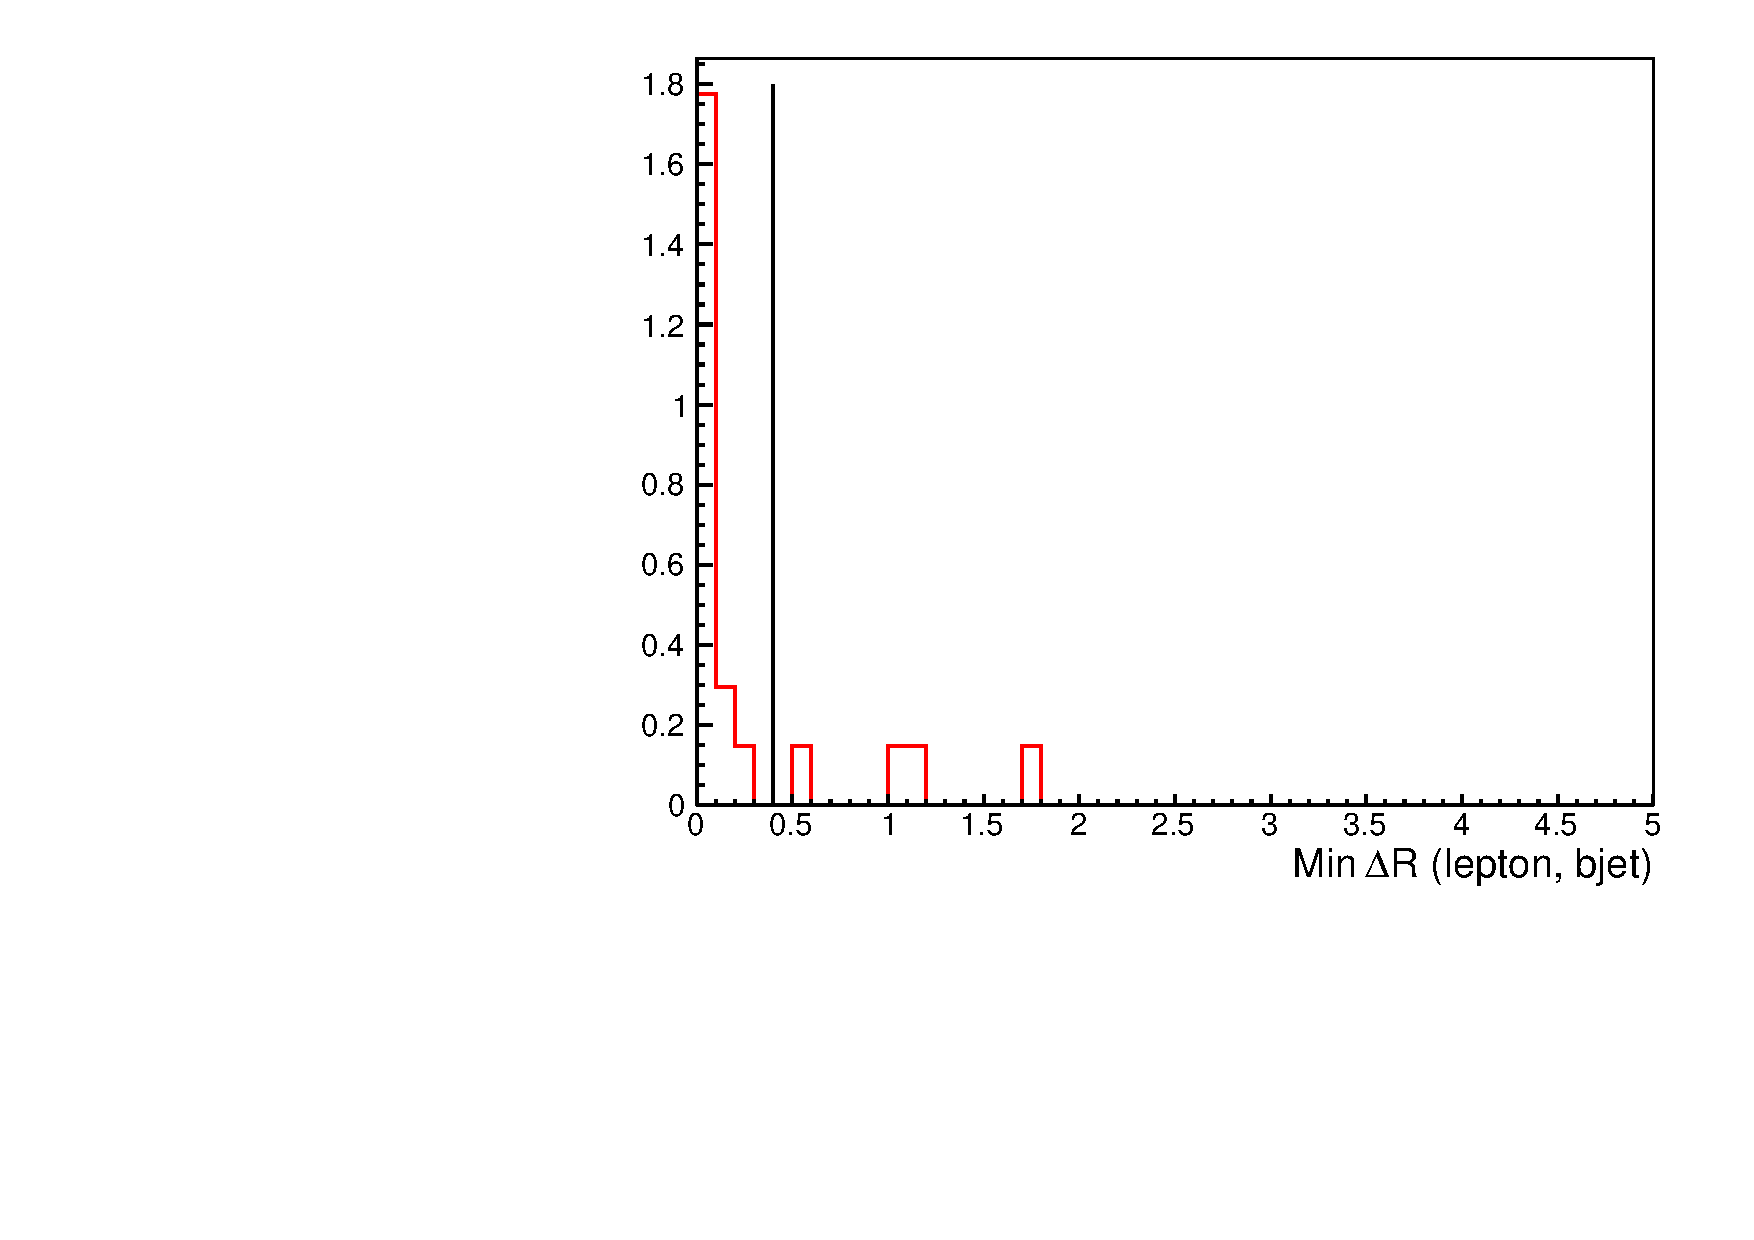
\includegraphics[width=0.6\linewidth, height=0.4\linewidth]{figs/bjetlepton.pdf}
%%\caption{ Minimum $\Delta R$ between the lepton and the b-tag jet in \ttbar\ decays.\label{fig:ttbar_residual}}
%%\end{center}
%%\end{figure}

{\bf This section is missing two things. 
First, we will add a \met\ vs $H_T$ plot that shows the data and
one of the models overlayed. 
Second, we will add a summary of the events we see. 
}


 




